\chapter{A neurális hálózat betanítása}
Ebben a fejezetben részletezem a felismeréshez használt neurális hálózat betanítását, a betanításhoz a Tensorflow\cite{tensorflow_autodiff} könyvtárat fogom használni Python programozási nyelven. A betanítás után a neurális háló model egy fájlba kerül mentésre, amelyet a felismerő program betölt és használ golyók osztályozására.

\section{Könyvtárak importálása}
A betanításhoz szükség van néhány külső könyvtár használatára, ezek a \ref{cod:classifier_imports} kódrészletben láthatóak.

\begin{codewrapper}
\begin{lstlisting}[language=Python, numbers=left, caption={A betanításhoz használt könyvtárak importálása.}, label={cod:classifier_imports}]
import random
import numpy as np

import tensorflow as tf
from tensorflow import keras

import cv2
import os
\end{lstlisting}
\end{codewrapper}

\par A \lstinline{random} és \lstinline{numpy} könyvtárak az adatkészlet betöltéséhez kerülnek felhasználásra főként, a \lstinline{numpy} könyvtárral lehetséges nagyméretű tömbökön műveletek gyors végrehajtása, mátrix műveletek elvégzése, a \lstinline{random} könyvtárral a betöltött adatokat lehet keverni, ami fontos a háló megfelelő betanításához.
\par Szükség van még az előzőekben említett Tensorflow könyvtár importálására, ez az 5. és 6. sorban történik meg, továbbá az OpenCV könyvtárra a képek betöltéséhez és HSV konvertálásához. Végül, a mappák eléréséhez az \lstinline{os} könyvtár kerül felhasználásra.

\section{Az adatkészlet betöltése}
Az adatkészlet betöltésénél a cél, hogy legyen egy betanítási és egy tesztelési adatkészlet, amelyek felépülnek egy golyóhoz tartozó kép adataiból és egy hozzájuk tartozó címkéből, amely a golyó színét adja meg. A tanítási adatkészlet a nevéből adódóan a hálózat betanításához használatos, a tesztelési adatkészlet a betanítási folyamat ellenőrzésére szolgál.
\par Ahhoz hogy el lehessen készíteni ezeket az adatkészleteket először be kell tölteni az adatokat. Az adatok színenként csoportosított mappákban helyezkednek el, azomban egyes mappákban nem egyenlő mennyiségű adat áll rendelkezésre, ezért az adatok betöltése előtt meg kell állapítani a lekevesebb adatot tartalmazó mappát, majd ez alapján betölteni a többit. A méret megállapítását a \ref{cod:smallest_dataset} kódrészlet mutatja.

\begin{codewrapper}
\begin{lstlisting}[language=Python, numbers=left, caption={A legkevesebb elemmel rendelkező adatkészlet megállapítása.}, label={cod:smallest_dataset}]
directory = "./dataset"
classes = ["black", "blue", "brown", "green", "pink", "red", "white", "yellow"]

lengths = []
for class in classes:
    class_dir = directory + "/" + class
    files = os.listdir(class_dir)
    lengths.append(len(files))

size = min(lengths)
\end{lstlisting}
\end{codewrapper}

\par Ebben a kódrészletben először meg kell adni az elérési útvonalat a \lstinline{directory} változóval, továbbá az egyes színekhez tartozó mappák listáját a \lstinline{classes} listával. A \lstinline{lengths} lista fogja tárolni az egyes mappákban található adatok mennyiségét.
\par A mennyiségek kiszámolásához először a \lstinline{class_dir} változóba belekerül a tényleges elérési útvonal, ez például a \lstinline{classes} tömb 0. elemének esetében '\lstinline{./dataset/black}' értéket vesz fel. A mappában található fájlok listáját a \lstinline{os.listdir} függvény adja meg az elérési útvonal alapján, majd a listát beleteszi a \lstinline{files} tömbbe. A fájlok mennyisége ezután a \lstinline{lengths} listához adódik hozzá a kód 8. sorában látható módon. A mennyiség lista legkisebb elemét a \lstinline{min} függvény adja meg, az eredmény a \lstinline{size} változóban kerül tárolásra.
\par A legkisebb adatkészlet megállapítása után következik az adatok betöltése, a betöltéshez használt kód a \ref{cod:dataset_load} kódrészletben látható.

\begin{codewrapper}
\begin{lstlisting}[language=Python, numbers=left, caption={Az adatkészlet betöltése.}, label={cod:dataset_load}]
images = []
labels = []

for class in classes:
    class_dir = directory + "/" + class
    files = os.listdir(class_dir)

    random.shuffle(files)
    files = files[:size]

    for file in files:
        bgr = cv2.imread(class_dir + "/" + file, cv2.IMREAD_COLOR)
        hsv = cv2.cvtColor(bgr, cv2.COLOR_BGR2HSV)

        combined = np.append(bgr, hsv, axis=2)
        images.append(combined)
        labels.append(np.where(classes == class))
\end{lstlisting}
\end{codewrapper}

\par Itt a fájlok listájának megszerzéséig a folyamat megegyezik a \ref{cod:smallest_dataset} kódrészletben használt módszerrel, a különbségek a 8. sortól kezdődnek, itt a \lstinline{random.shuffle} függvény segítségével a \lstinline{files} tömb összekeverése történik meg, majd a tömb mérete levágásra kerül az előzőekben kiszámolt legkisebb adatkészlet méretére. A levágás után a szkript végighalad a fájlokon, azokat betöltve a \lstinline{cv2.imread} függvény\cite{opencv_docs} segítségével, amelynek első paramétere a betöltendő kép elérési útja, a második pedig a betöltés módja, amely jelen esetben \lstinline{cv2.IMREAD_COLOR}, ez azt adja meg, hogy a kép színes BGR formátumban kerüljön betöltésre.
\par A betöltött kép a \lstinline{bgr} változóba kerül, a képet a felismeréshez konvertálni kell HSV formátumra, ezt a \lstinline{cv2.cvtColor} függvény teszi meg, amelynek meg kell adni az átalakítani kívánt képet és az átalakítás módjat (\lstinline{cv2.COLOR_BGR2HSV}), amely jelen esetben a HSV konverziót jelzi. A HSV konverzióról bővebben a \ref{section:megv_asztal_kontur} részben lesz szó.
\par A konverzió után a BGR és HSV értékek intenzitás értékei összefűzésre kerülnek a \lstinline{np.append} függvény segítségével, itt a képek megadásával meg kell adni, hogy az összefűzés a képek mátrixának 3. dimenzióján történjen, ezt a \lstinline{axis=2} paraméter adja meg. Az összefűzés után a kezdetben létrehozott \lstinline{images} tömbbe kerül bele az összefűzőtt kép, a hozzá tartozó címke pedig a \ref{cod:smallest_dataset} kódrészletben található \lstinline{classes} tömbben található index alapján kerül hozzáfűzésre a \lstinline{labels} tömbhöz.
\par A következő lépés a betanítási és tesztelési adatkészletek különválasztása, ennek a folyamata a \ref{cod:train_test_separate} kódrészletben található.

\begin{codewrapper}
\begin{lstlisting}[language=Python, numbers=left, caption={A tanítási és tesztelési adatkészletek elkülönítése.}, label={cod:train_test_separate}]
images = np.array(images)
labels = np.array(labels).reshape(-1)

labels = keras.utils.to_categorical(labels)

border = int(size * 0.8)

train_images = images[:border]
train_labels = labels[:border]
test_images = images[border:]
test_labels = labels[border:]
\end{lstlisting}
\end{codewrapper}

\par A kódrészletben először az \lstinline{images} és \lstinline{labels} változókat numpy tömbre alakítjom a \lstinline{np.array} függvény segítségével, majd a \lstinline{labels} tömböt átalakítom bináris osztály mátix formájába a \lstinline{keras.utils.to_categorical} függvény\cite{tensorflow_docs} segítségével. Ez a konvertálás mindössze annyit jelent, hogy egy adott címke például \lstinline{3} bináris reprezentációban lesz feltüntetve egy \lstinline{[0, 0, 0, 1, 0, 0, 0, 0]} tömb formájában, feltéve ha 8 db címke áll rendelkezésre. Ezt az átalakítást szokták one-hot kódolásnak is nevezni\cite{harris2012digital}. Az egyes címkék kódolt változatai a \ref{tab:one_hot_labels} táblázatban láthatóak.

\begin{table}[!ht]
    \caption{A golyók szín szerint, és azok azonosítói.}
    \label{tab:one_hot_labels}
	\footnotesize
	\centering
	\begin{tabular}{ l c }
		\toprule
		Golyó címkéje & One-hot kódolt reprezentáció \\
		\midrule
		fekete      & [1, 0, 0, 0, 0, 0, 0, 0]\\
        kék         & [0, 1, 0, 0, 0, 0, 0, 0]\\
        barna       & [0, 0, 1, 0, 0, 0, 0, 0]\\
        zöld        & [0, 0, 0, 1, 0, 0, 0, 0]\\
        rózsaszín   & [0, 0, 0, 0, 1, 0, 0, 0]\\
        piros       & [0, 0, 0, 0, 0, 1, 0, 0]\\
        fehér       & [0, 0, 0, 0, 0, 0, 1, 0]\\
        sárga       & [0, 0, 0, 0, 0, 0, 0, 1]\\
		\bottomrule
	\end{tabular}
\end{table}

\par A kódolást követően egy határérték kerül kiszámolásra a \lstinline{border} változóba, ez szimplán megadja, hogy az elemek mekkora része legyen tanításra és mekkora legyen tesztelésre felhasználva. A határérték egy egész szám formájában adja meg az elválasztás pontját, majd a szétválasztás a 8. - 11. sorban látható módon megy végbe. Az elválasztás végeztével az adatkészlet készen áll a betanítási folyamatokra.

\section{A neurális hálózat felépítése és betanítása}
A neurális hálózat több rétegből épül fel, ezek közül az első réteg egy konvolúciós réteg. Ez a konvolúciós réteg közvetlenül fogadja a felismerésre szánt képet, amely jelen esetben egy 5 x 5 méretű kernelt használ 8 különböző konvolúció elkészítéséhez. A konvolúciók elkészítése után egy ún. Max-Pool eljárással azok léképezése történik, az eljárás egy 2 x 2 méretű kernellel dolgozik, minden ilyen kernel elemeit kombinálja egy értékbe, ennek következtében a konvolúciók mátrixának mérete felére csökken. Ez a művelet a teljesítmény növelésében játszik szerepet a neurális hálózat kapcsolatainak leszűkítésével.
\par A konvolúció és Max-Pool rétegek után az adatok egy ún. 'lapítás' (flatten) műveleten esnek át ez az elemeket egy egydimenziós vektorba helyezi. A vektorrá alakítás után következik még két, egy 18 és egy 8 csomópontból álló réteg, ezek a lapított réteghez hasonlóan szintén egydimenziós vektorok. A két réteg méretét próbálgatás útján állapítottam meg a megfelelő sebesség és pontosság eléréséhez.
\par Az utolsó réteg egy kimeneti réteg, amely megadja a bemenetként adott golyóról, hogy azt egyes színek milyen mértékben reprezentálják. Ez egy 8 elemű \ref{tab:one_hot_labels} táblázatban látott one-hot értékhez hasonló lista formájában mutatkozik. A neurális hálózat felépítését a \ref{fig:neural_network_model} ábra szemlélteti, hálózat konfigurálásához használt kód pedig a \ref{cod:neural_network_model_def} kódrészletben látható.

\begin{figure}[!ht]
    \centering
    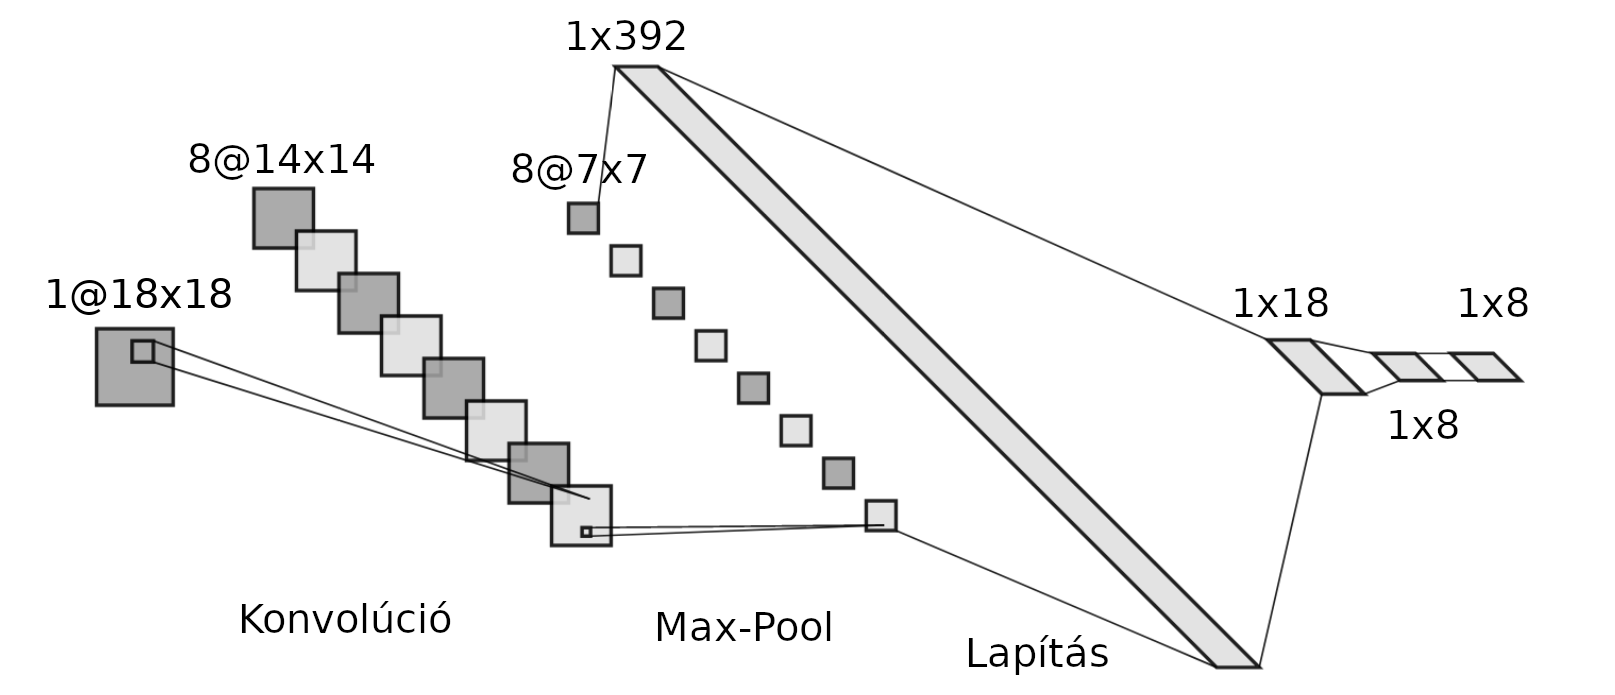
\includegraphics[width=140mm, keepaspectratio]{figures/neural_network_model.png}
    \caption[A neurális hálózat modeljének felépítése.]{A neurális hálózat modeljének felépítése.\cite{alexlenail}}
    \label{fig:neural_network_model}
\end{figure}

\begin{codewrapper}
\begin{lstlisting}[language=Python, numbers=left, caption={A neurális hálózat konfigurálása.}, label={cod:neural_network_model_def}]
model = keras.models.Sequential([
    keras.layers.Conv2D(8, (5, 5), activation="relu", input_shape=(18, 18, 6)),
    keras.layers.MaxPool2D((2, 2)),
    keras.layers.Flatten(),
    keras.layers.Dense(18, activation="relu"),
    keras.layers.Dense(8, activation="relu"),
    keras.layers.Dense(8)
])
\end{lstlisting}
\end{codewrapper}

\par A \ref{cod:neural_network_model_def} kódrészletben az első sorban a model létrehozása történik, ezt a \lstinline{keras.models.Sequential} függvény\cite{chollet2015keras,tensorflow_docs} teszi meg. A modell a \lstinline{model} változóban kerül tárolásra. A létrehozáshoz használt függvény belsejében található lista az egyes rétegeket adja meg, ezek közül az első a konvolúciós réteg, amelyet a \lstinline{keras.layers.Conv2D} függvény\cite{chollet2015keras,tensorflow_docs} ad meg. A függvény paraméterei megadják a konvolúciók számát, a használt kernel méretét, az aktivációs függvényt és a bemeneti mátrix alakját. Az aktivációs függvény megadja, hogy adott bemenetekre hogyan reagáljon, és milyen kimenetet adjon a neurális hálózat egy csomópontja\cite{hinkelmannneural}. Ennél a megoldásnál egy ún. ReLU (Rectified Linear Unit) aktivációs függvény kerül felhasználásra, amelyet a \ref{for:RELU} egyenlet\cite{RELU2010} ír le.

\begin{equation}
    f(x) =
    \begin{cases}
        0 & ,\text{ha}\ x\le0 \\
        x & ,\text{ha}\ x>0
    \end{cases}
    \label{for:RELU}
\end{equation}

\par Az egyenlet alapján, ha az aktivációs függvény bemeneti értéke 0 alatt van, akkor a kimeneti 0, ha 0 felett van, akkor pedig a bemeneti érték megegyezik a kimeneti értékkel. A függvényt a \ref{fig:relu_function} ábra mutatja koordináta rendszerben.

\begin{figure}[!ht]
    \centering
    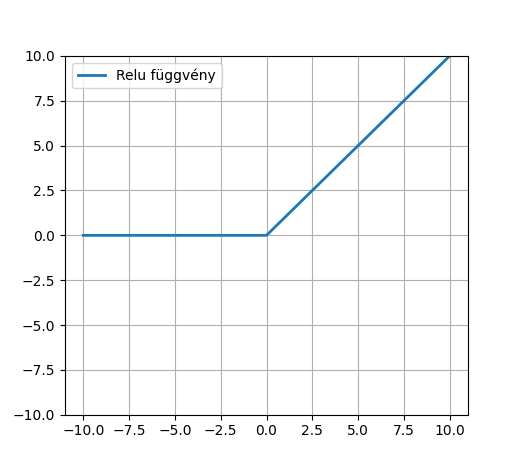
\includegraphics[width=100mm, keepaspectratio]{figures/relu_function.png}
    \caption{ReLU aktivációs függvény ábrázolása.}
    \label{fig:relu_function}
\end{figure}

\par A \ref{cod:neural_network_model_def} kódrészlethez visszatérve a hálózat második rétege a \lstinline{keras.layers.MaxPool2D} függvénnyel\cite{chollet2015keras,tensorflow_docs} kerül megadásra, itt az egyetlen paraméter a kernel mérete. A max-pool réteg után következik a lapítást végző réteg, ezt a \lstinline{keras.layers.Flatten} függvény\cite{chollet2015keras,tensorflow_docs} adja meg, majd ezután következik még két teljesen kapcsol (Dense) réteg, amelyeket a \lstinline{keras.layers.Dense} függvény\cite{chollet2015keras,tensorflow_docs} biztosít. A teljesen kapcsolt rétegek függvényének bemenetei a réteg nagysága és aktivációs függvénye, ami ebben az esetben is a ReLU aktivációs függvény. Az utolsó kimeneti réteg is az előzőekhez hasonló teljesen kapcsolt réteg, viszont itt nincs szükség aktivációs függvényre.
\par A neurális hálózat rétegeinek megadása után be kell állítani a veszteségfüggvényt és az optimalizáló algoritmust, majd ezután megezdődhet a háló betanítása és kiértékelése az adatkészletek segítségével. Az említett konfigurálás programkód formájában a \ref{cod:train_network} kódrészletben szerepel.

\begin{codewrapper}
\begin{lstlisting}[language=Python, numbers=left, caption={A neurális hálózat betanítása.}, label={cod:train_network}]
loss = keras.losses.CategoricalCrossentropy(from_logits=True)
optimizer = keras.optimizers.Adam(learning_rate=0.0001)

model.compile(loss=loss, optimizer=optimizer)
model.fit(train_images, train_labels, epochs=20, batch_size=5)
model.evaluate(test_images, test_labels, batch_size=5)

model.add(keras.layers.Softmax())

model.save("classifier.h5")
\end{lstlisting}
\end{codewrapper}

\par Itt a veszteségfüggvényt a \lstinline{keras.losses.CategoricalCrossentropy} függvény adja meg\cite{chollet2015keras,tensorflow_docs}, ami kereszt entrópiát\cite{rubinstein2004cross} használ a veszteség kiszámolásához. A veszteség ezesetben megadja, hogy egy adott bemenet alapján a kimeneti érték mennyiben különbözik az elvárt kimeneti értéktől. Az optimalizáló algoritmus a \lstinline{keras.optimizers.Adam} függvénnyel\cite{chollet2015keras,tensorflow_docs} adható meg, ez egy gyakran használt optimalizáló algoritmust alkalmaz, amelyet Adam optimalizálónak neveznek, ez az algorimus egy gradiens süllyedéses módszerrel közelíti a kimeneti értéket az elvárt értékhez a veszteségfüggvény segítségével\cite{adam2014}. A \lstinline{learning_rate} paraméterrel megadható a tanítás sebessége, amely a gradiens süllyedés módszer lépéseinek nagyságával befolyásolja a sebességet. Túl nagy tanítási sebesség a pontosság veszítéséhez vezethet, azomban túl kicsi sebesség viszont a tanításhoz szükséges időt nagymértékben növelheti.
\par A veszteség függvény és optimalizáló beállítása után a hálózat fordítását a \lstinline{model.compile} függvénnyel\cite{chollet2015keras,tensorflow_docs} lehet elvégezni, amelynek paraméterként meg kell adni a veszteségfüggvényt és optimalizálót, ezután a betanítást a \lstinline{model.fit} függvénnyel\cite{chollet2015keras,tensorflow_docs} lehet megtenni, amelynek meg kell adni a betanításhoz szükséges adatokat és azok címkéjeit, továbbá meg kell adni egy \lstinline{epochs} paramétert, ez megadja, hogy tanítás során az algoritmus hányszor iteráljon végig a teljes adatkészleten, továbbá meg kell adni egy \lstinline{batch_size} paramétert, ami megadja, hogy mekkora adatcsoportonként frissítse az értékeit a gradiens süllyedéses algoritmus. Tanítás közben a hálózat vesztesége, avagy a kapott eredmény és várt eredmény eltérése folyamatosan csökken, ezt a \ref{fig:loss_metrics} ábra szemlélteti.

\begin{figure}[!ht]
    \centering
    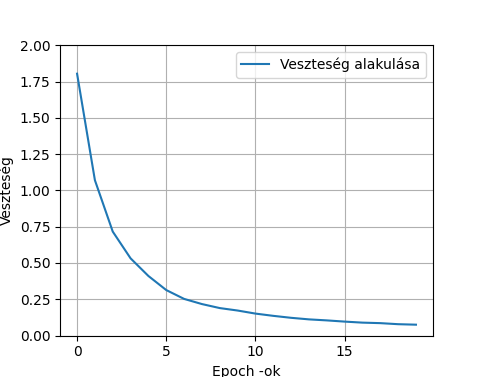
\includegraphics[width=110mm, keepaspectratio]{figures/loss_metrics.png}
    \caption{A veszteség alakulása a tanítási folyamat során.}
    \label{fig:loss_metrics}
\end{figure}

\par A tanítás után a kiértékelést a \lstinline{model.evaluate} függvénnyel\cite{chollet2015keras,tensorflow_docs} lehet elvégezni, ennek bemenetként a teszt adatkészlet és címkék kerülnek megadásra, továbbá a tanításhoz hasonlóan az adatcsoportok mérete.
\par A betanítás után a modelhez egy Softmax réteg kerül hozzáadásra a programkód 8. sorában látható módon, ez a réteg a kimeneti értékeket átalakítja valószínűség formájába, ami azt jelenti, hogy egy jósolt érték 8 elemből álló listájánál az értékek összege mindíg 1 értéket ad.
\par A hálózat betanítása után annak elmentése egy fájlba a \lstinline{model.save} függvénnyel\cite{chollet2015keras,tensorflow_docs} lehetséges, amelynek paraméterül a mentéshez használt nevet kell megadni. A mentés után a modellt a felismerő programba könnyedén be lehet tölteni, és osztályozni a golyókat színük alapján.